\documentclass[11pt,a4paper,spanish]{book}
\usepackage{estilo_unir-1}
\usepackage{tikz}
\usetikzlibrary{positioning, arrows.meta, decorations.pathmorphing}



%---------------------------
%título del trabajo y autor
%---------------------------
\title{Oscilador armónico cuántico (OAC)}
\author{Nombre y Apellidos}
\date{diaXXX de mesXXX de 2023}
\profesor{Rodrigo Gil-Merino y Rubio}

%---------------------------
%marges
%---------------------------
%\usepackage[margin=1.9cm]{geometry}
%---------------------------
%---------------------------
%---------------------------
%---------------------------
\begin{document}
\renewcommand{\listfigurename}{Índice de figuras}
\renewcommand{\listtablename}{Índice de tablas}
\renewcommand{\contentsname}{Índice de contenidos}
\renewcommand{\figurename}{Figura}
\renewcommand{\tablename}{Tabla} 

\maketitle

\frontmatter
\tableofcontents
\listoffigures %atención, quitar si no hay figuras!!!
\listoftables %atención, quitar si no hay tablas!!!

\chapter{Resumen}
Aquí se introducirá un breve resumen en español del trabajo realizado (extensión máxima: 150 palabras). Este resumen debe incluir el objetivo o propósito de la investigación, la metodología, los resultados y las conclusiones (obviamente, todo muy resumido, pero así se sabe de un vistazo lo que se va uno a encontrar a continuación).\\


{\bf Palabras clave:} se deben incluir de 3 a 5 palabras claves en español (pueden ser conceptos formados por más de una palabra)

\chapter{Abstract}
Aquí debe introducirse la versión en {\bf inglés} del Resumen anterior.\\


{\bf Keywords:} se deben incluir de 3 a 5 palabras claves en inglés  (pueden ser conceptos formados por más de una palabra)




\mainmatter
\chapter{Introducción}

El oscilador armónico cuántico (OAC) constituye, junto con el átomo de hidrógeno, el modelo fundamental de la mecánica cuántica. Su importancia trasciende lo pedagógico: es el fundamento físico de las principales plataformas de computación cuántica actuales y la base de los únicos códigos de corrección de errores que han superado experimentalmente el punto de equilibrio. Este trabajo establece las conexiones entre las predicciones históricas del modelo (1900-1963), su validación experimental reciente (2020-2025), y su implementación en arquitecturas de procesamiento cuántico.

\begin{itemize}
\item Motivación.\\
\textbf{Identificación del problema:} A pesar de que el oscilador armónico cuántico se encuentar en prácticamente todos los textos de mecánica cuántica, su tratamiento suele enfocarse a ejercicios de aplicación matemática sin establecer conexiones explícitas con las tecnologías cuánticas actuales. Existe una brecha entre la comprensión teórica del modelo y su reconocimiento como fundamento operativo de las plataformas de computación cuántica más avanzadas. Esta desconexión impide apreciar cómo el modelo del OAC sigue siendo la base de los desarrollos experimentales recientes que están transformando la corrección de errores cuánticos.\\

\textbf{Justificación de su importancia:} Comprender con cierto nivel de detalle el oscilador armónico cuántico (OAC) es fundamental para cualquier profesional que trabaje en computación cuántica o física. El OAC no es simplemente un ejercicio didáctico: es el lenguaje operativo de circuit QED \citep{blais2021}, la física subyacente de los modos motacionales en iones atrapados \citep{cirac1995, leibfried2003}, y el espacio de codificación de los códigos bosónicos que han superado el punto de equilibrio en corrección de errores \cite{sivak2023, ni2023, reglade2024}. Entender este modelo proporciona las herramientas conceptuales y matemáticas necesarias para entender literatura técnica especializada, evaluar arquitecturas de procesadores cuánticos, y contribuir al diseño de nuevas implementaciones.\\

\textbf{Contribución esperada:} Este trabajo busca establecer una base conceptual sólida y articulada del oscilador armónico cuántico que sirva como plataforma para estudios avanzados en la maestría y para aplicaciones prácticas en computación cuántica. Específicamente, pretende: \textbf{(1)} conectar los conceptos teóricos con su realización experimental moderna; \textbf{(2)} proporcionar un catálogo actualizado de referencias primarias que permita profundizar en aspectos específicos según necesidades futuras; \textbf{(3)} demostrar que el OAC no es solo historia de la física, sino ingeniería cuántica contemporánea, permitiendo comprender desarrollos futuros; y \textbf{(4)} establecer un vocabulario técnico base (operadores escalera, estados coherentes, función de Wigner, códigos bosónicos).\\

Comprender los nuevos desarrollos que se han dado en el período 2020-2025, requiere entender y dominar el OAC como fundamento, objetivo central de este trabajo. Este periodo ha marcado una transición con desarrollos como: los códigos bosónicos han superado el punto de equilibrio en corrección de errores \cite{sivak2023, ni2023}, cat qubits han alcanzado tiempos de bit-flip superiores a 10 segundos \cite{reglade2024}, sistemas optomecánicos han enfriado osciladores a 0.04 fonones desde temperatura ambiente \cite{dania2025} y creado estados gato en resonadores de 16 microgramos \cite{bild2023}, y resonadores fonónicos han verificado directamente la cuantización de energía \cite{arrangoiz2019, hou2024}.\\ 

\item Planteamiento del Trabajo\\
Esta actividad presenta el oscilador armónico cuántico (OAC) como fundamento teórico y tecnológico de las arquitecturas de computación cuántica actuales, estableciendo conexiones entre predicciones históricas (1900-1963), validación experimental (2020-2025), e implementación en plataformas de procesamiento cuántico. \\

El análisis traza la evolución desde Planck \citep{planck1901} hasta Glauber \citep{glauber1963a}, explicando algunos fundamentos matemáticos a nivel básico, catalogando validaciones experimentales 2020-2025 en circuitos superconductores \citep{sivak2023, ni2023, reglade2024}, iones atrapados \citep{hou2024}, sistemas optomecánicos \citep{dania2025, bild2023}, y resonadores fonónicos \citep{arrangoiz2019, wollack2022}. Se establecen conexiones directas con computación cuántica mediante transmons \citep{koch2007, blais2021}, iones atrapados \citep{cirac1995, bruzewicz2019}, códigos bosónicos \citep{gkp2001, ofek2016, brady2024}, y CVQC fotónica \citep{braunstein2005, madsen2022}, proyectando la hoja de ruta tecnológica 2025-2035 con arquitecturas emergentes y desafíos críticos \citep{liu2024, eickbusch2024, chamberland2022}.

\item Estructura del Trabajo\\
La primera sección muestra el progreso histórico desde los orígenes clásicos \citep{hooke1678, lagrange1788, hamilton1834} hasta las formulaciones cuánticas completas de Planck \citep{planck1901}, Einstein \citep{einstein1907}, Heisenberg \citep{heisenberg1925}, Schrödinger \citep{schrodinger1926b}, Dirac \citep{dirac1930}, y Glauber \citep{glauber1963a}, mostrando cómo el OAC sirvió como base para la construcción de los conceptos centrales de la mecánica cuántica.\\

La segunda sección presenta el formalismo matemático: hamiltoniano y relaciones de conmutación, espectro de energía cuantizado, operadores escalera y estructura algebraica bosónica, estados coherentes, y función de Wigner. Este tratamiento enfatiza comprensión física con referencias a textos fundamentales \citep{griffiths2018, sakurai2020, cohentannoudji2019, gerry2004, nielsen2010}, definiendo el vocabulario téncico que reaparecerá en secciones posteriores.\\

La tercera sección documenta realizaciones experimentales 2020-2025 organizadas por plataforma: circuitos superconductores superando break-even \citep{sivak2023, ni2023, reglade2024, putterman2025}, iones atrapados demostrando interferencia de fonones \citep{hou2024, burd2024, park2024}, sistemas optomecánicos alcanzando régimen cuántico macroscópico \citep{dania2025, bild2023, piotrowski2023}, y resonadores fonónicos verificando cuantización \citep{arrangoiz2019, wollack2022, qiao2023}. Esta sección muestra que el OAC no es una abstracción teórica sino un componente tecnológico funcional.\\

La cuarta sección establece conexiones directas con computación cuántica mediante las aplicaciones del OCA: transmons como OAC anarmónicos en circuit QED \citep{koch2007, blais2021, krantz2019}, iones atrapados explotando modos motacionales como bus cuántico \citep{cirac1995, molmer1999, bruzewicz2019}, códigos bosónicos (cat, GKP, binomiales) para corrección de errores hardware-efficient \citep{gkp2001, ofek2016, michael2016, brady2024}, CVQC fotónica \citep{braunstein2005, madsen2022, bourassa2021}, y Kerr-cat qubits \citep{grimm2020, hajr2024}.\\ 

La quinta sección proyecta la hoja de ruta 2025-2035 en tres fases temporales, analiza arquitecturas emergentes \citep{liu2024, eickbusch2024, chamberland2022}, e identifica cinco desafíos tecnológicos críticos que determinan la viabilidad de estas proyecciones.


\end{itemize}




\chapter{Contexto y estado del Oscilador armónico cuántico}\label{contexto}

El oscilador armónico cuántico (OAC) es, junto con el átomo de hidrógeno, el modelo más importante de toda la mecánica cuántica. Su relevancia trasciende lo pedagógico: constituye el fundamento físico de las principales plataformas de computación cuántica actuales, desde qubits superconductores hasta iones atrapados y computación cuántica fotónica.
El oscilador armónico cuántico es un modelo fundamental que describe partículas en un potencial parabólico con energía cuantizada (valores discretos). Sus características principales incluyen:
\begin{itemize}
	\item \textbf{Niveles energéticos:} Igualmente espaciados, con separación constante (hv)
	\item \textbf{Energía de punto cero:} El estado base tiene energía no nula debido a fluctuaciones cuánticas
	\item \textbf{Funciones de onda:} Estados estacionarios descritos por funciones de Hermite con factor gaussiano
	\item \textbf{Principio de incertidumbre:} Posición y momento están sujetos a las restricciones de Heisenberg
\end{itemize}

Este modelo es esencial para comprender vibraciones atómicas en cristales, óptica cuántica y teoría cuántica de campos, siendo una base fundamental para el estudio de sistemas cuánticos más complejos.


\chapter{Objetivos}

\section {Objetivo General}
Presentar el oscilador armónico cuántico (OAC) como fundamento teórico y tecnológico de las arquitecturas de computación cuántica actuales, estableciendo conexiones explícitas entre las predicciones del modelo (1900-1963), su validación experimental reciente (2020-2025), y su implementación en plataformas de procesamiento cuántico.

\section {Objetivos específicos}

\begin{itemize}
	\item Trazar la evolución histórica y teórica del OAC desde la cuantización de Planck (1900) hasta los estados coherentes de Glauber (1963), explicando los fundamentos matemáticos básicos (hamiltoniano, operadores escalera, función de Wigner).
	\item Catalogar las validaciones experimentales del OAC en plataformas diversas (circuitos superconductores, iones atrapados, sistemas optomecánicos, resonadores fonónicos) durante 2020-2025, verificando predicciones como cuantización de energía, energía de punto cero y negatividad de función de Wigner.
	\item Proyectar la hoja de ruta tecnológica 2025-2035 para procesadores cuánticos basados en osciladores, argumentando que la concatenación de códigos bosónicos con códigos discretos constituye la vía más prometedora hacia computación cuántica tolerante a fallos escalable.
\end{itemize} 



\chapter{Desarrollo del Trabajo}


\section{Desarrollo histórico del oscilador armónico cuántico}

La historia del oscilador armónico cuántico (OAC) es inseparable de la historia de la mecánica cuántica misma. Desde la cuantización ad hoc de Planck en 1900 hasta el formalismo riguroso de Glauber en 1963, este modelo sirvió como base para la construcción y definición de los conceptos centrales de la teoría: cuantización de energía, energía de punto cero, operadores no conmutativos, y estados coherentes. \\

Cada avance conceptual —la mecánica matricial de Heisenberg, la ecuación de onda de Schrödinger, el método algebraico de Dirac— se validó primero resolviendo el oscilador armónico cuántico. Esta sección traza ese recorrido, identificando los autores y teorías que transformaron un modelo clásico del siglo XVII en el fundamento de las tecnologías cuánticas del siglo XXI.

\subsection*{Orígenes clásicos}
El concepto de oscilador armónico tiene raíces en la mecánica clásica del siglo XVII. Robert Hooke formuló su ley de fuerza restauradora lineal (Ut tensio, sic vis — "como la extensión, así la fuerza") en su obra \cite{hooke1678}. La formalización matemática se completó con la mecánica analítica de Lagrange \citep{lagrange1788} y Hamilton \citep{hamilton1834, hamilton1835} , estableciendo el hamiltoniano clásico $H = \frac{p^2}{2m} + \frac{1}{2}m\omega^2 x^2$ como modelo universal para oscilaciones pequeñas alrededor de cualquier punto de equilibrio estable.\\

Para finales del siglo XIX, el oscilador armónico clásico era el paradigma central de sistemas oscilatorios en mecánica, acústica y electrodinámica. Su importancia radicaba en que cualquier potencial V(x) cerca de un mínimo puede aproximarse como cuadrático mediante una expansión de Taylor~\ref{sec:taylor} , haciendo del oscilador armónico una aproximación universal.\\

\begin{figure}[h]
    \centering
    % timeline_oac.tex
% Versión con máximo espaciado y sin superposiciones

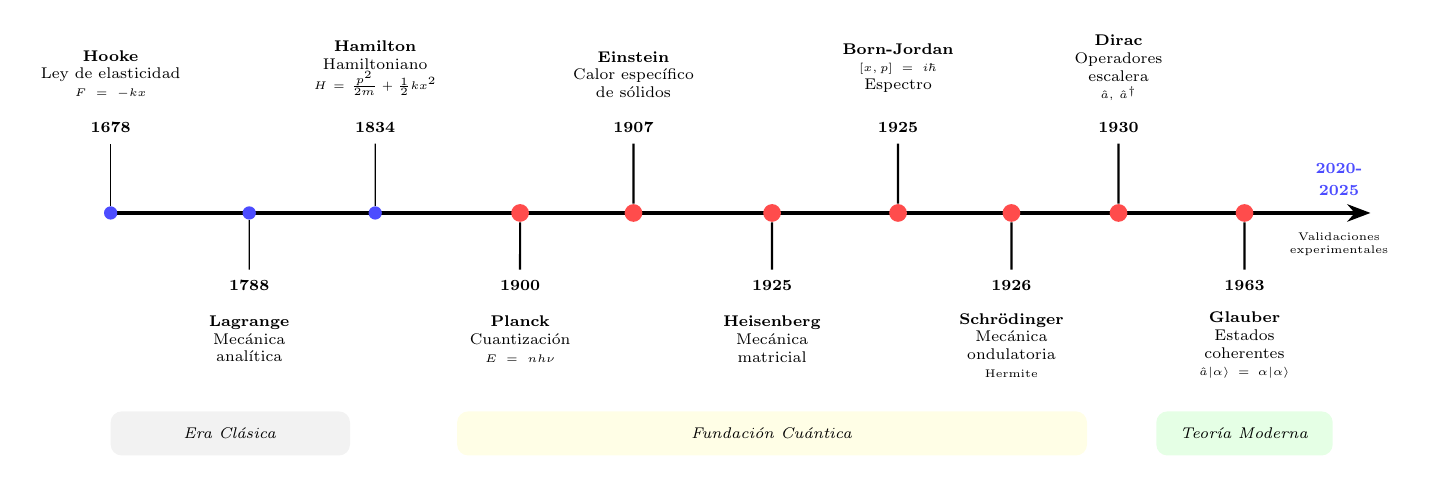
\begin{tikzpicture}[
    % Estilos para los nodos
    evento/.style={circle, fill=blue!70, inner sep=2pt, minimum size=6pt},
    evento_mayor/.style={circle, fill=red!70, inner sep=2.5pt, minimum size=8pt},
    texto/.style={font=\scriptsize, text width=2.4cm, align=center},
    año/.style={font=\scriptsize\bfseries},
    scale=0.8, transform shape
    ]
    
    % Línea temporal principal (aún más larga)
    \draw[line width=1.2pt, -Stealth] (0,0) -- (20,0);
    
    % Etiquetas de períodos (fondo) - más separadas
    \node[fill=gray!10, rounded corners, minimum width=3.8cm, minimum height=0.7cm] at (1.9, -3.5) {\scriptsize\textit{Era Clásica}};
    \node[fill=yellow!10, rounded corners, minimum width=10cm, minimum height=0.7cm] at (10.5, -3.5) {\scriptsize\textit{Fundación Cuántica}};
    \node[fill=green!10, rounded corners, minimum width=2.8cm, minimum height=0.7cm] at (18, -3.5) {\scriptsize\textit{Teoría Moderna}};
    
    % PERÍODO CLÁSICO
    % Hooke 1678
    \node[evento] (hooke) at (0,0) {};
    \draw (hooke) -- (0,1.1);
    \node[año] at (0,1.35) {1678};
    \node[texto] at (0,2.2) {\textbf{Hooke}\\ Ley de elasticidad\\ {\tiny $F = -kx$}};
    
    % Lagrange 1788
    \node[evento] (lagrange) at (2.2,0) {};
    \draw (lagrange) -- (2.2,-0.9);
    \node[año] at (2.2,-1.15) {1788};
    \node[texto] at (2.2,-2) {\textbf{Lagrange}\\ Mecánica\\ analítica};
    
    % Hamilton 1834
    \node[evento] (hamilton) at (4.2,0) {};
    \draw (hamilton) -- (4.2,1.1);
    \node[año] at (4.2,1.35) {1834};
    \node[texto] at (4.2,2.3) {\textbf{Hamilton}\\ Hamiltoniano\\ {\tiny $H = \frac{p^2}{2m} + \frac{1}{2}kx^2$}};
    
    % PERÍODO CUÁNTICO INICIAL
    % Planck 1900
    \node[evento_mayor] (planck) at (6.5,0) {};
    \draw[thick] (planck) -- (6.5,-0.9);
    \node[año] at (6.5,-1.15) {1900};
    \node[texto] at (6.5,-2) {\textbf{Planck}\\ Cuantización\\ {\tiny $E = nh\nu$}};
    
    % Einstein 1907
    \node[evento_mayor] (einstein) at (8.3,0) {};
    \draw[thick] (einstein) -- (8.3,1.1);
    \node[año] at (8.3,1.35) {1907};
    \node[texto] at (8.3,2.2) {\textbf{Einstein}\\ Calor específico\\ de sólidos};
    
    % DÉCADA PRODIGIOSA - MÁXIMO ESPACIADO
    % Heisenberg 1925
    \node[evento_mayor] (heisenberg) at (10.5,0) {};
    \draw[thick] (heisenberg) -- (10.5,-0.9);
    \node[año] at (10.5,-1.15) {1925};
    \node[texto] at (10.5,-2) {\textbf{Heisenberg}\\ Mecánica\\ matricial};
    
    % Born-Jordan 1925 (bien separado de Heisenberg)
    \node[evento_mayor] (born) at (12.5,0) {};
    \draw[thick] (born) -- (12.5,1.1);
    \node[año] at (12.5,1.35) {1925};
    \node[texto] at (12.5,2.3) {\textbf{Born-Jordan}\\ {\tiny $[x,p] = i\hbar$}\\ Espectro};
    
    % Schrödinger 1926
    \node[evento_mayor] (schrodinger) at (14.3,0) {};
    \draw[thick] (schrodinger) -- (14.3,-0.9);
    \node[año] at (14.3,-1.15) {1926};
    \node[texto] at (14.3,-2.1) {\textbf{Schrödinger}\\ Mecánica\\ ondulatoria\\ {\tiny Hermite}};
    
    % Dirac 1930
    \node[evento_mayor] (dirac) at (16,0) {};
    \draw[thick] (dirac) -- (16,1.1);
    \node[año] at (16,1.35) {1930};
    \node[texto] at (16,2.3) {\textbf{Dirac}\\ Operadores\\ escalera\\ {\tiny $\hat{a}$, $\hat{a}^\dagger$}};
    
    % TEORÍA MODERNA
    % Glauber 1963
    \node[evento_mayor] (glauber) at (18,0) {};
    \draw[thick] (glauber) -- (18,-0.9);
    \node[año] at (18,-1.15) {1963};
    \node[texto] at (18,-2.1) {\textbf{Glauber}\\ Estados\\ coherentes\\ {\tiny $\hat{a}|\alpha\rangle = \alpha|\alpha\rangle$}};
    
    % Época actual (indicador)
    \node[font=\scriptsize\bfseries, text=blue!70] at (19.5, 0.7) {2020-};
    \node[font=\scriptsize\bfseries, text=blue!70] at (19.5, 0.35) {2025};
    \node[font=\tiny, text width=1.8cm, align=center] at (19.5, -0.5) {Validaciones\\experimentales};
    
\end{tikzpicture}
    \caption{Línea temporal del desarrollo del oscilador armónico cuántico desde los fundamentos clásicos (1678) hasta la teoría moderna (1963) y las validaciones experimentales recientes (2020-2025). Fuente propia.}
    \label{fig:timeline_oac}
\end{figure}


\subsection*{La cuantización de Planck (1900)}
La transición de lo clásico a lo cuántico surgió del \textbf{problema de la radiación del cuerpo negro}. Las leyes de \cite{wien1896} y \cite{rayleigh1900, jeans1905} fallaban en diferentes rangos espectrales, y la segunda predecía una divergencia ultravioleta catastrófica. Max Planck presentó  el 19 de octubre de 1900 ante la Sociedad Alemana de Física \citep{planck1901} su derivación teórica, que requería que la energía de estos osciladores estuviera restringida a múltiplos discretos de una unidad fundamental: $E = n\hbar\nu$. El 14 de diciembre de 1900, Planck había llegado a una conclusión algo radical: los osciladores que comprenden el cuerpo negro y que re-emiten la energía radiante que incide sobre ellos no pueden absorber esta energía de forma continua, tan solo en cantidades discretas, o cuantos de energía.\\

\textbf{Significado:} Los resonadores de Planck eran precisamente osciladores armónicos con energía cuantizada. La introducción de la constante $h$ marcó el nacimiento de la teoría cuántica, aunque Planck mismo fue cauteloso sobre la interpretación física de la cuantización.



\subsection*{Einstein y el calor específico de los sólidos (1907)}
\textbf{Albert Einstein} fue el primero en tomar la hipótesis de cuantización en serio y aplicarla más allá de la radiación. En \cite{einstein1907}, modeló un sólido cristalino como una colección de osciladores armónicos cuánticos independientes, todos vibrando a la misma frecuencia. Su modelo~\ref{sec:einstein} predecía correctamente que el calor específico se anula exponencialmente cuando T → 0, en contraste con la ley clásica de Dulong-Petit.

\subsection*{Heisenberg y la mecánica matricial (1925)}
En el verano de 1925, \textbf{Werner Heisenberg} \citep{heisenberg1925} construyó una nueva mecánica basada exclusivamente en cantidades observables ~\ref{sec:heisenberg}. El oscilador armónico (específicamente, un oscilador anarmónico) fue el sistema de prueba principal de su paper fundacional.

El trabajo de Heisenberg sobre el oscilador armónico fue:

\begin{itemize}
	\item La \textbf{primera formulación completa y autoconsistente} de la mecánica cuántica
	\item La primera derivación rigurosa del espectro del OAC sin hipótesis ad hoc
	\item El origen del \textbf{principio de incertidumbre}: la no-conmutación implica que $x$ y $p$ no pueden tener valores simultáneos definidos
	\item La base conceptual de la \textbf{teoría cuántica de campos}, donde operadores (no funciones de onda) son fundamentales
\end{itemize}

Schrödinger demostró posteriormente (1926) que su mecánica ondulatoria era matemáticamente equivalente a la mecánica matricial, pero el formalismo de operadores de Heisenberg resultó más fundamental para el desarrollo posterior de la física cuántica.

\textbf{Nota:} Heisenberg trabajó inicialmente con un oscilador \emph{anarmónico} (con términos cúbicos en el potencial) como sistema de prueba más general, demostrando que su método funcionaba incluso cuando no había solución exacta conocida.\\


\textbf{Max Born y Pascual Jordan} reconocieron la estructura matricial y formalizaron la mecánica de Heisenberg ~\ref{sec:born}, estableciendo la relación de conmutación canónica $pq - qp = (\frac{\hslash}{i})\mathbb{I}$ y derivando por primera vez el espectro de energía $E_n = (n + \frac{1}{2})\hslash\omega$, incluyendo la energía de punto cero $\frac{1}{2}\hslash\omega$.\\

El método de Born-Jordan-Heisenberg (algebráico) es notable porque:

\begin{enumerate}
	\item \textbf{No requiere resolver ecuaciones diferenciales} — es puramente algebraico
	\item \textbf{Proporciona el espectro completo} incluyendo la energía de punto cero automáticamente
	\item \textbf{Introduce los operadores $a$ y $a^\dagger$} que son fundamentales en toda la física cuántica moderna
	\item \textbf{Es generalizable} — el mismo método funciona para cualquier sistema con álgebra de conmutadores conocida
\end{enumerate}

Este formalismo se convirtió en la base de la \textbf{segunda cuantización} y la teoría cuántica de campos, donde los operadores de creación ($a^\dagger$) y aniquilación ($a$) crean y destruyen partículas (fotones, fonones, electrones, etc.).\\


\subsection*{Schrödinger y la mecánica ondulatoria (1926)}
\textbf{Erwin Schrödinger}  desarrolló una formulación equivalente pero completamente diferente~\ref{sec:taylor}. En la segunda de sus cuatro comunicaciones tituladas "Quantisierung als Eigenwertproblem"  \cite{schrodinger1926b}, aplicó su ecuación de onda al oscilador armónico y obtuvo las soluciones en términos de \textbf{polinomios de Hermite}, confirmando el espectro $E_n = (n + 1/2)\hslash\omega$\\

\begin{figure}[h]
    \centering
    
\includegraphics[width=0.6\linewidth]{Figures/HarmOsziFunktionen.png}
    \caption{Funciones de onda de un Oscilador armónico cuántico. Licencia: Public domain o CC-BY}
    \label{fig:HarmOsziFunktionen}
\end{figure}

En física contemporánea, especialmente en computación cuántica, se usa predominantemente el formalismo de operadores (método algebraico), mientras que las funciones de onda se emplean para visualización y cálculos específicos.

\subsection*{El método algebraico de Dirac: operadores de creación y aniquilación (1930)}
\textbf{Paul Dirac} desarrolló un método algebraico \citep{dirac1925} que evita resolver ecuaciones diferenciales~\ref{sec:dirac}, introduciendo los operadores escalera $[a, a^\dagger]$. La factorización del hamiltoniano como $H = \hbar\omega\left(a^\dagger a + \frac{1}{2}\right)$ y la derivación puramente algebraica del espectro se convirtieron en el enfoque pedagógico estándar y, crucialmente, en la plantilla para la teoría cuántica de campos.\\

El método de Dirac se convirtió en el \textbf{enfoque pedagógico estándar} porque:

\begin{enumerate}
	\item Es conceptualmente más simple que resolver ecuaciones diferenciales
	\item Proporciona intuición física directa (subir/bajar niveles de energía)
	\item Se generaliza inmediatamente a sistemas de múltiples osciladores
	\item Es la base natural para entender fotones, fonones, y otras cuasipartículas
	\item Conecta directamente con el formalismo de información cuántica\\
\end{enumerate}

El formalismo de operadores escalera de Dirac es el lenguaje estándar de:

\begin{itemize}
	\item \textbf{Circuit QED}: El hamiltoniano de Jaynes-Cummings usa explícitamente $\hat{a}$ y $\hat{a}^\dagger$ para fotones en cavidades \citep{blais2021}
	\item \textbf{Códigos bosónicos}: Estados de Fock $|n\rangle$ son la base para códigos GKP y binomiales \citep{gkp2001, michael2016}
	\item \textbf{Estados coherentes}: Definidos como autoestados de $\hat{a}$ \citep{glauber1963a}
	\item \textbf{CVQC}: Operadores de desplazamiento y compresión se expresan en términos de $\hat{a}$ y $\hat{a}^\dagger$ \citep{braunstein2005}
\end{itemize}

El método algebraico de Dirac, desarrollado en 1930 para resolver el oscilador armónico, es hoy el marco conceptual de la computación cuántica basada en osciladores.


\subsection*{Los estados coherentes de Glauber (1963)}
\textbf{Roy J. Glauber} proporcionó el marco completo de la óptica cuántica para estados coherentes \citep{glauber1963a}, definidos como autoestados del operador de aniquilación $\hat{a}|\alpha\rangle = \alpha|\alpha\rangle$. Estos estados representan el análogo cuántico más cercano al comportamiento clásico oscilatorio.\\

Glauber recibió el Premio Nobel de Física 2005 por este trabajo, que estableció la óptica cuántica como disciplina rigurosa.\\


Los estados coherentes son fundamentales en múltiples aplicaciones de computación cuántica:

\textbf{Cat codes (códigos gato):} \citep{ofek2016, reglade2024}
Superposiciones de estados coherentes $|\alpha\rangle \pm |-\alpha\rangle$ que codifican qubits lógicos con protección exponencial contra errores de bit-flip.

\textbf{Control de iones atrapados:} \citep{leibfried2003}
La luz láser usada para manipular qubits iónicos se describe como estados coherentes del campo electromagnético.

\textbf{Computación cuántica de variables continuas (CVQC):} \citep{braunstein2005, bourassa2021}
Estados coherentes son la base computacional natural. El operador desplazamiento $\hat{D}(\alpha)$ es una puerta cuántica fundamental.

\textbf{Códigos GKP:} \citep{gkp2001}
Construcciones basadas en superposiciones periódicas de estados coherentes desplazados en espacio de fase.

\textbf{Teleportación cuántica de variables continuas:} \citep{braunstein2005}
Usa estados coherentes comprimidos (squeezed) como recurso de entrelazamiento.\\

Los estados coherentes de Glauber, concebidos para describir luz láser en 1963, son hoy bloques fundamentales de arquitecturas de computación cuántica que han alcanzado tiempos de coherencia superiores a 10 segundos \cite{reglade2024}.


\section{Fundamentos matemáticos y físicos}

El formalismo matemático del oscilador armónico cuántico combina elegancia teórica con utilidad práctica inmediata. Esta sección presenta los cinco pilares conceptuales del modelo: 

\begin{itemize}
	\item El hamiltoniano cuantizado.
	\item Los niveles de energía discretos.
	\item Los operadores de creación y aniquilación.
	\item Los estados coherentes.
	\item La representación en espacio de fase mediante la función de Wigner.
\end{itemize}

El tratamiento de estos fundamentes es a un nivel básico, enfatizando la comprensión física de cada elemento y sus implicaciones para computación cuántica, sin profundizar en derivaciones matemáticas exhaustivas. Cada concepto se acompaña de referencias específicas a textos de referencia para quien desee mayor rigor. El objetivo es establecer el vocabulario y las herramientas que reaparecerán constantemente en las secciones posteriores: experimentales y de aplicaciones.



\subsection*{El hamiltoniano del oscilador armónico cuántico}
Pendiente

\subsection*{Niveles de energía cuantizados}
Pendiente

\subsection*{Operadores escalera (creación y aniquilación)}
Pendiente

\subsection*{Estados coherentes}
Pendiente

\subsection*{Representación en el espacio de fase}
Pendiente


\section{Realizaciones experimentales modernas (2020-2025)}
El período 2020-2025 marca una transición cualitativa en la física del oscilador armónico cuántico: de validar predicciones fundamentales a implementarlo como componente tecnológico funcional.\\

Esta sección documenta los experimentos más significativos organizados por plataforma física (circuitos superconductores, iones atrapados y sistemas optomecánicos), mostrando cómo cada predicción teórica de la Sección 4.2 —cuantización de energía, energía de punto cero, estados coherentes, negatividad de función de Wigner— ha sido verificada experimentalmente con alta precisión.\\ 


\subsection*{Circuitos superconductores: el OAC como qubit lógico}

Los resonadores de microondas superconductores son realizaciones físicas directas del oscilador armónico cuántico. Estos dispositivos, operando a temperaturas cercanas al cero absoluto, se comportan exactamente como el OAC teórico: tienen niveles de energía cuantizados $E_n = \hbar\omega(n + \frac{1}{2})$ y se describen mediante los operadores de creación y aniquilación $\hat{a}^\dagger$ y $\hat{a}$ introducidos por Dirac.\\

El período 2020-2025 ha marcado un hito histórico: por primera vez, experimentos lograron que qubits lógicos codificados en estos osciladores tuvieran \textbf{mayor tiempo de vida} que sus componentes físicos individuales. Este logro, llamado \textbf{superar el punto de equilibrio (break-even)}, demuestra que la corrección de errores cuánticos realmente funciona.\\

Los experimentos 2020-2025 en circuitos superconductores han validado experimentalmente predicciones fundamentales del OAC:

\begin{itemize}
	\item Los estados de Fock $|n\rangle$ con número definido de fotones se pueden preparar y manipular
	\item Los estados coherentes $|\alpha\rangle$ de Glauber se comportan exactamente como predijo la teoría
	\item Las superposiciones de estados coherentes (cat states) exhiben propiedades cuánticas macroscópicas
	\item La función de Wigner muestra negatividad genuina en estados no-clásicos
	\item El espacio de Hilbert infinito del OAC permite estrategias de corrección de errores imposibles con qubits binarios
\end{itemize}

Muy importante, tres experimentos independientes \citep{sivak2023, ni2023, reglade2024} superaron el punto de equilibrio usando estrategias diferentes, todas basadas en aprovechar la estructura del OAC. Esto refleja que el oscilador armónico cuántico ha pasado de ser un modelo pedagógico a ser la plataforma física líder para computación cuántica tolerante a fallos.

\subsubsection{Estados GKP superando break-even (Yale, 2023)} 

\textbf{Qué hicieron:} El grupo de Yale \citep{sivak2023} codificó un qubit lógico usando estados especiales del oscilador armónico llamados \textbf{estados GKP} (Gottesman-Kitaev-Preskill). Estos estados son patrones periódicos en el espacio de fase del oscilador, construidos como superposiciones de estados coherentes.

\textbf{Qué validaron del OAC:} Los estados GKP solo existen porque el oscilador tiene un espacio de Hilbert infinito-dimensional. Usan explícitamente los operadores $\hat{a}$ y $\hat{a}^\dagger$ para construir estas superposiciones especiales que protegen contra errores.

\textbf{Resultado clave:} El qubit lógico vivió 2.0 ms, mientras que el resonador físico solo vivía 1.0 ms. Por primera vez, agregar corrección de errores \emph{mejoró} (no empeoró) la vida de la información cuántica.

\textbf{Por qué importa:} Demuestra que el espacio infinito del OAC permite proteger información cuántica de formas imposibles con sistemas de solo dos niveles.


\subsubsection{Códigos binomiales superando break-even (2023)}

\textbf{Qué hicieron:} \cite{ni2023} codificaron un qubit lógico usando \textbf{estados de Fock} del oscilador (estados con número definido de fotones $|0\rangle, |1\rangle, |2\rangle, \ldots$) combinados con coeficientes binomiales especiales.

\textbf{Qué validaron del OAC:} Los estados de Fock son los autoestados naturales del operador número $\hat{N} = \hat{a}^\dagger\hat{a}$. Este experimento demuestra que podemos controlar y manipular estos estados individuales del oscilador con precisión cuántica.

\textbf{Resultado clave:} El qubit lógico alcanzó 0.6 ms de vida, superando los ~0.3 ms de sus componentes físicos.

\textbf{Por qué importa:} Confirma que múltiples estrategias de codificación sobre el OAC pueden superar break-even, no solo una.

\subsubsection{Cat qubit con 10 segundos de coherencia (Alice \& Bob / ENS Paris, 2024)}

\textbf{Qué hicieron:} \cite{reglade2024} crearon un \textbf{cat qubit} — un qubit codificado en superposiciones de estados coherentes del oscilador. El nombre viene de que estos estados son análogos cuánticos al gato de Schrödinger: superposiciones de estados macroscópicamente distinguibles.

\textbf{Qué validaron del OAC:} Estos experimentos confirman que los estados coherentes — introducidos por \cite{glauber1963a} para describir luz láser — realmente existen en osciladores físicos y se comportan como predijo la teoría.

\textbf{Resultado clave:} Tiempo de vida contra errores de bit-flip mayor a \textbf{10 segundos}, una mejora de 10,000 veces respecto a intentos anteriores. 

\textbf{Por qué importa:} Demuestra que el comportamiento predicho de estados coherentes (protección exponencial contra ciertos errores) se verifica experimentalmente. Diez segundos es un tiempo enorme en computación cuántica — suficiente para millones de operaciones.


\subsection*{Iones atrapados: modos motacionales como osciladores armónicos}
En la computación cuántica con iones atrapados, átomos individuales (típicamente Be$^+$, Ca$^+$, Yb$^+$, Sr$^+$) se confinan mediante campos electromagnéticos en el vacío. Cada ion tiene dos tipos de grados de libertad cuánticos:

\begin{itemize}
	\item \textbf{Estados internos}: Niveles electrónicos del átomo que funcionan como qubit (|0⟩ y |1⟩)
	\item \textbf{Estados motacionales}: Vibración del ion en la trampa, que se comporta como un OAC con hamiltoniano $\hat{H} = \hbar\omega_m(\hat{a}^\dagger\hat{a} + \frac{1}{2})$
\end{itemize}

Los \textbf{modos motacionales} son cruciales porque actúan como \textbf{bus cuántico}: permiten que dos iones distantes interactúen intercambiando fonones (cuantos de vibración), exactamente como lo propusieron \cite{cirac1995}. Esta es la segunda arquitectura líder de computación cuántica junto con circuitos superconductores.\\

La frecuencia típica de los modos motacionales es $\omega_m/2\pi \sim 1-10$ MHz, mucho más baja que transiciones electrónicas ($\sim 10^{14}$ Hz). Los experimentos 2020-2025 han demostrado control cuántico sin precedentes de estos osciladores armónicos vibratorios.\\

Los experimentos con iones atrapados 2020-2025 han validado que los modos motacionales son osciladores armónicos cuánticos perfectos:

\begin{itemize}
	\item Los fonones se comportan como bosones idénticos con interferencia cuántica
	\item Los estados coherentes de Glauber existen en vibraciones mecánicas, no solo en luz
	\item El control cuántico de estos osciladores permite arquitecturas de computación cuántica escalables
\end{itemize}

Estos osciladores operan a frecuencias $\sim$ MHz (seis órdenes de magnitud más bajas que fotones ópticos), demostrando que la física del OAC es universal e independiente de la escala de energía. Los iones atrapados representan la segunda plataforma líder de computación cuántica comercial, validando que múltiples realizaciones físicas del OAC son viables para tecnología.



\subsubsection{Interferencia cuántica de fonones individuales (NIST, 2024)}

\textbf{Qué hicieron:} \cite{hou2024} demostraron el análogo del experimento de \cite{hong1987} clásico de óptica cuántica~\ref{sec:hong}, pero usando \textbf{fonones} (cuantos de vibración) en lugar de fotones. Dos modos motacionales de iones distintos se hicieron interferir en un ``beam splitter fonónico''.

\textbf{Qué validaron del OAC:} Los fonones se comportan exactamente como excitaciones bosónicas del OAC:
\begin{itemize}
	\item Los estados de Fock de vibración $|0\rangle, |1\rangle, |2\rangle, \ldots$ existen y son manipulables
	\item Los operadores $\hat{a}^\dagger$ y $\hat{a}$ crean y destruyen fonones individuales
	\item Los fonones exhiben interferencia cuántica de dos partículas, como predicen los operadores bosónicos
\end{itemize}

\textbf{Resultado clave:} Observación de \textbf{bunching cuántico} — cuando dos fonones idénticos llegan simultáneamente al beam splitter, siempre salen juntos por el mismo puerto (nunca se separan). Este es el efecto HOM, firma de estadística bosónica.

\textbf{Por qué importa:} Demuestra que vibraciones cuantizadas de iones se comportan idénticamente a fotones en sus propiedades cuánticas. Los fonones son realizaciones del OAC tan válidas como los fotones. Esto valida el uso de modos motacionales como bus cuántico en procesadores de iones.




\subsection*{Sistemas optomecánicos: el OAC en escala mesoscópica}
Los sistemas optomecánicos estudian la interacción entre luz y objetos mecánicos, donde la presión de radiación de fotones puede enfriar, controlar y medir el movimiento cuántico de osciladores mecánicos. A diferencia de los resonadores superconductores (fotones confinados) o iones atrapados (átomos individuales), estos experimentos demuestran el OAC en \textbf{objetos mesoscópicos} — sistemas que contienen miles de millones de átomos pero aún exhiben comportamiento cuántico.\\

La pregunta fundamental que estos experimentos responden es: \textbf{¿Hasta qué escala de tamaño y masa funcionan las predicciones del OAC?} Los resultados 2020-2025 han sido muy llamativos: desde nanopartículas levitadas en el vacío hasta membranas de 16 microgramos, todos siguiendo exactamente $\hat{H} = \hbar\omega(\hat{a}^\dagger\hat{a} + \frac{1}{2})$.\\

Los experimentos optomecánicos 2020-2025 han llevado las validaciones del OAC hacia el régimen mesoscópico:

\begin{itemize}
	\item La cuantización $E_n = \hbar\omega(n + \frac{1}{2})$ funciona en objetos con $10^{14}$ átomos
	\item La energía de punto cero existe mediblemente en osciladores de microgramos
	\item Los estados coherentes y cat states de Glauber pueden prepararse en membranas macroscópicas
	\item El estado fundamental es alcanzable sin criogenia mediante aislamiento suficiente

\end{itemize}

Estos resultados responden una pregunta fundamental: \textbf{¿Hay un límite de tamaño para la mecánica cuántica?} La respuesta experimental es no — el límite es de \emph{decoherencia}, no de masa. Si un oscilador puede aislarse suficientemente de su entorno, exhibirá comportamiento cuántico independientemente de su tamaño, validando que el OAC es una descripción universal aplicable desde electrones hasta objetos macroscópicos.

\subsubsection{Enfriamiento cuántico a temperatura ambiente (ETH Zurich, 2025)}

\textbf{Qué hicieron:} \cite{dania2025} enfriaron una nanopartícula de sílice levitada ópticamente en el vacío hasta alcanzar el estado fundamental del oscilador — específicamente, $\langle n \rangle = 0.04$ fonones — trabajando \textbf{a temperatura ambiente} (300 K) en lugar de requerir criogenia.

\textbf{Qué validaron del OAC:} 
\begin{itemize}
	\item La cuantización de energía $E_n = \hbar\omega(n + \frac{1}{2})$ se aplica a objetos macroscópicos, no solo sistemas microscópicos
	\item La energía de punto cero $E_0 = \frac{1}{2}\hbar\omega$ existe en osciladores mesoscópicos
	\item El número promedio de fonones $\langle n \rangle$ es medible y controlable incluso cerca del estado fundamental
\end{itemize}

\textbf{Resultado clave:} $\langle n \rangle = 0.04 \pm 0.01$ fonones — el oscilador mecánico está $96\%$ del tiempo en su estado fundamental $|0\rangle$, a pesar de que la energía térmica a 300 K es $k_B T \sim 10^{14}$ veces mayor que $\hbar\omega$.

\textbf{Por qué importa:} 
\begin{enumerate}
	\item Demuestra que la física cuántica funciona a temperatura ambiente si el oscilador está suficientemente aislado
	\item Valida la existencia de energía de punto cero en objetos ``visibles''
	\item Plantea alternativas a sensores cuánticos sin criogenia
\end{enumerate}

\subsubsection{Estados gato de Schrödinger en 16 microgramos (ETH Zurich, 2023)}

\textbf{Qué hicieron:} \cite{bild2023} crearon \textbf{estados gato de Schrödinger} — superposiciones cuánticas de dos estados coherentes macroscópicamente distinguibles — en una membrana mecánica de silicio de \textbf{16 microgramos}. Esta membrana contiene aproximadamente $10^{14}$ átomos de silicio moviéndose coherentemente en una superposición cuántica.\\

\textbf{Qué validaron del OAC:} 
\begin{itemize}
	\item Los estados coherentes $|\alpha\rangle$ introducidos por Glauber existen en osciladores mecánicos macroscópicos
	\item Se pueden crear superposiciones cuánticas de estados macroscópicamente distinguibles (separación $\sim 100$ veces el estado fundamental)
	\item El principio de superposición cuántica se aplica a objetos con $10^{14}$ átomos
\end{itemize}


\textbf{Por qué importa:} 
\begin{enumerate}
	\item Valida el escenario del gato de Schrödinger en un objeto casi macroscópico
	\item Demuestra que no hay límite de masa para comportamiento cuántico — solo límite de aislamiento del entorno
\end{enumerate}



\section{Aplicaciones en computación cuántica}

El oscilador armónico cuántico no es un componente auxiliar de la computación cuántica: es su infraestructura fundamental. Esta sección explora de una manera general, las implementaciones físicas del OAC en la computación cuántica. Más allá de estas implementaciones, esta sección analiza cómo el espacio de Hilbert infinito-dimensional del OAC se explota activamente en códigos bosónicos (cat, GKP, binomiales) para corrección de errores hardware-efficient, demostrando que las únicas arquitecturas que han superado experimentalmente el punto de equilibrio son precisamente aquellas que codifican qubits lógicos dentro de osciladores individuales. El OAC pasa así de abstracción matemática a estrategia de protección de información cuántica.


\subsection*{Definir hasta qué nivel de detalle llegamos, ya que es un tema complejo que sobrepasa mi concimiento actual}
Pendiente

\section{Perspectivas futuras y desafíos (2025-2035)}
Los códigos bosónicos se posicionan como la estrategia líder para corrección de errores cuánticos escalable, habiendo superado experimentalmente el punto de equilibrio donde otros enfoques aún no lo logran. Esta sección proyecta la evolución esperada del campo mediante una hoja de ruta en tres fases: demostración de módulos tolerantes a fallos a pequeña escala (2025-2027), integración de decenas de qubits bosónicos corregidos en procesadores (2027-2030), y despliegue de computadores cuánticos tolerantes a fallos a gran escala usando osciladores como primera capa de corrección (2030-2035). 

Finalmente, se identifican los cinco desafíos tecnológicos críticos que determinan si esta hoja de ruta se materializa: coherencia del oscilador, errores de ancilla, control multimodal escalable, calidad de estados GKP, e integración de componentes.

\subsection*{Los códigos bosónicos como estrategia líder de corrección de errores}
Pendiente

\subsection*{Arquitecturas emergentes basadas en osciladores}
Pendiente

\subsection*{Desafíos tecnológicos principales}
Pendiente


\chapter{Conclusiones}

Las Conclusiones es otra parte muy IMPORTANTE de la memoria. Deben ser muy clara. Si es posible se pueden itemizar o, mejor, poner un párrafo por idea con un pequeño título ilustrativo.

\addcontentsline{toc}{chapter}{Bibliografía}
\begin{thebibliography}{a}

%% ORÍGENES CLÁSICOS Y PRE-CUÁNTICOS

\bibitem[Hooke(1678)]{hooke1678} Hooke, R. (1678) \emph{Lectures de Potentia Restitutiva, or of Spring. Explaining the Power of Springing Bodies}. John Martyn, London.

\bibitem[Lagrange(1788)]{lagrange1788} Lagrange, J.L. (1788) \emph{Mécanique analytique}. Desaint, Paris.

\bibitem[Hamilton(1834)]{hamilton1834} Hamilton, W.R. (1834) On a General Method in Dynamics. \textit{Philosophical Transactions of the Royal Society}, Part I, 247--308.

\bibitem[Hamilton(1835)]{hamilton1835} Hamilton, W.R. (1835) Second Essay on a General Method in Dynamics. \textit{Philosophical Transactions of the Royal Society}, Part I, 95--144.

\bibitem[Wien(1896)]{wien1896} Wien, W. (1896) Über die Energievertheilung im Emissionsspectrum eines schwarzen Körpers. \textit{Annalen der Physik}, \textbf{294}(8), 662--669. DOI: 10.1002/andp.18962940803

\bibitem[Rayleigh(1900)]{rayleigh1900} Rayleigh, J. W. S. (1900) Remarks upon the Law of Complete Radiation. \textit{Philosophical Magazine}, \textbf{49}, 539--540.

\bibitem[Jeans(1905)]{jeans1905} Jeans, J.H. (1905) XI. On the Partition of Energy between Matter and Aether. \textit{The London, Edinburgh, and Dublin Philosophical Magazine and Journal of Science}, \textbf{10}, 91--98.

\bibitem[Debye(1912)]{debye1912} Debye, P. (1912) Zur Theorie der spezifischen Wärmen. \textit{Annalen der Physik}, \textbf{39}(4), 789--839. DOI: 10.1002/andp.19123441404


%% PAPERS SEMINALES HISTÓRICOS

\bibitem[Planck(1901)]{planck1901} Planck, M. (1901) Über das Gesetz der Energieverteilung im Normalspektrum. \textit{Annalen der Physik}, \textbf{309}(3), 553--563. DOI: 10.1002/andp.19013090310

\bibitem[Einstein(1907)]{einstein1907} Einstein, A. (1907) Die Plancksche Theorie der Strahlung und die Theorie der spezifischen Wärme. \textit{Annalen der Physik}, \textbf{22}, 180--190. DOI: 10.1002/andp.19063270110

\bibitem[Heisenberg(1925)]{heisenberg1925} Heisenberg, W. (1925) Über quantentheoretische Umdeutung kinematischer und mechanischer Beziehungen. \textit{Zeitschrift für Physik}, \textbf{33}, 879--893. DOI: 10.1007/BF01328377

\bibitem[Born \& Jordan(1925)]{born1925} Born, M. y Jordan, P. (1925) Zur Quantenmechanik. \textit{Zeitschrift für Physik}, \textbf{34}, 858--888.

\bibitem[Born et al.(1926)]{bornheisenberg1926} Born, M., Heisenberg, W. y Jordan, P. (1926) Zur Quantenmechanik II. \textit{Zeitschrift für Physik}, \textbf{35}, 557--615.

\bibitem[Schrödinger(1926a)]{schrodinger1926a} Schrödinger, E. (1926) Quantisierung als Eigenwertproblem (Erste Mitteilung). \textit{Annalen der Physik}, \textbf{384}(4), 361--376. DOI: 10.1002/andp.19263840404

\bibitem[Schrödinger(1926b)]{schrodinger1926b} Schrödinger, E. (1926) Quantisierung als Eigenwertproblem (Zweite Mitteilung). \textit{Annalen der Physik}, \textbf{384}(6), 489--527. DOI: 10.1002/andp.19263840602

\bibitem[Schrödinger(1926c)]{schrodinger1926c} Schrödinger, E. (1926) Der stetige Übergang von der Mikro- zur Makromechanik. \textit{Naturwissenschaften}, \textbf{14}, 664--666. DOI: 10.1007/BF01507634

\bibitem[Dirac(1925)]{dirac1925} Dirac, P.A.M. (1925) The Fundamental Equations of Quantum Mechanics. \textit{Proceedings of the Royal Society of London A}, \textbf{109}, 642--653.

\bibitem[Dirac(1927)]{dirac1927} Dirac, P.A.M. (1927) The Quantum Theory of the Emission and Absorption of Radiation. \textit{Proceedings of the Royal Society of London A}, \textbf{114}(767), 243--265.

\bibitem[Dirac(1930)]{dirac1930} Dirac, P.A.M. (1930) \emph{The Principles of Quantum Mechanics}, 1st ed. Clarendon Press, Oxford.

\bibitem[Glauber(1963a)]{glauber1963a} Glauber, R.J. (1963) The Quantum Theory of Optical Coherence. \textit{Physical Review}, \textbf{130}(6), 2529--2539. DOI: 10.1103/PhysRev.130.2529

\bibitem[Glauber(1963b)]{glauber1963b} Glauber, R.J. (1963) Coherent and Incoherent States of the Radiation Field. \textit{Physical Review}, \textbf{131}(6), 2766--2788. DOI: 10.1103/PhysRev.131.2766

\bibitem[Sudarshan(1963)]{sudarshan1963} Sudarshan, E.C.G. (1963) Equivalence of Semiclassical and Quantum Mechanical Descriptions of Statistical Light Beams. \textit{Physical Review Letters}, \textbf{10}(7), 277--279. DOI: 10.1103/PhysRevLett.10.277

%% LIBROS DE TEXTO FUNDAMENTALES

\bibitem[Griffiths \& Schroeter(2018)]{griffiths2018} Griffiths, D.J. y Schroeter, D.F. (2018) \emph{Introduction to Quantum Mechanics}, 3rd ed. Cambridge University Press, Cambridge.

\bibitem[Sakurai \& Napolitano(2020)]{sakurai2020} Sakurai, J.J. y Napolitano, J. (2020) \emph{Modern Quantum Mechanics}, 3rd ed. Cambridge University Press, Cambridge.

\bibitem[Cohen-Tannoudji et al.(2019)]{cohentannoudji2019} Cohen-Tannoudji, C., Diu, B. y Laloë, F. (2019--2020) \emph{Quantum Mechanics}, Vols. 1--3, 2nd ed. Wiley-VCH, Weinheim.

\bibitem[Gerry \& Knight(2004)]{gerry2004} Gerry, C.C. y Knight, P.L. (2004) \emph{Introductory Quantum Optics}. Cambridge University Press, Cambridge.

\bibitem[Nielsen \& Chuang(2010)]{nielsen2010} Nielsen, M.A. y Chuang, I.L. (2010) \emph{Quantum Computation and Quantum Information}, 10th Anniversary ed. Cambridge University Press, Cambridge.

\bibitem[Schleich(2001)]{schleich2001} Schleich, W.P. (2001) \emph{Quantum Optics in Phase Space}. Wiley-VCH, Weinheim.

\bibitem[Case(2008)]{case2008} Case, W.B. (2008) Wigner functions and Weyl transforms for pedestrians. \textit{American Journal of Physics}, \textbf{76}(10), 937--946.

%% CIRCUIT QED Y QUBITS SUPERCONDUCTORES

\bibitem[Koch et al.(2007)]{koch2007} Koch, J., Yu, T.M., Gambetta, J., Houck, A.A., Schuster, D.I., Majer, J., Blais, A., Devoret, M.H., Girvin, S.M. y Schoelkopf, R.J. (2007) Charge-insensitive qubit design derived from the Cooper pair box. \textit{Physical Review A}, \textbf{76}, 042319.

\bibitem[Blais et al.(2004)]{blais2004} Blais, A., Huang, R.-S., Wallraff, A., Girvin, S.M. y Schoelkopf, R.J. (2004) Cavity quantum electrodynamics for superconducting electrical circuits: An architecture for quantum computation. \textit{Physical Review A}, \textbf{69}, 062320.

\bibitem[Blais et al.(2021)]{blais2021} Blais, A., Grimsmo, A.L., Girvin, S.M. y Wallraff, A. (2021) Circuit quantum electrodynamics. \textit{Reviews of Modern Physics}, \textbf{93}, 025005.

\bibitem[Wallraff et al.(2004)]{wallraff2004} Wallraff, A., Schuster, D.I., Blais, A., Frunzio, L., Huang, R.-S., Majer, J., Kumar, S., Girvin, S.M. y Schoelkopf, R.J. (2004) Circuit quantum electrodynamics: Coherent coupling of a single photon to a Cooper pair box. \textit{Nature}, \textbf{431}, 162--167.

\bibitem[Krantz et al.(2019)]{krantz2019} Krantz, P., Kjaergaard, M., Yan, F., Orlando, T.P., Gustavsson, S. y Oliver, W.D. (2019) A quantum engineer's guide to superconducting qubits. \textit{Applied Physics Reviews}, \textbf{6}, 021318.

%% IONES ATRAPADOS

\bibitem[Cirac \& Zoller(1995)]{cirac1995} Cirac, J.I. y Zoller, P. (1995) Quantum computations with cold trapped ions. \textit{Physical Review Letters}, \textbf{74}, 4091--4094.

\bibitem[Mølmer \& Sørensen(1999)]{molmer1999} Mølmer, K. y Sørensen, A. (1999) Multiparticle entanglement of hot trapped ions. \textit{Physical Review Letters}, \textbf{82}, 1835.

\bibitem[Bruzewicz et al.(2019)]{bruzewicz2019} Bruzewicz, C.D., Chiaverini, J., McConnell, R. y Sage, J.M. (2019) Trapped-ion quantum computing: Progress and challenges. \textit{Applied Physics Reviews}, \textbf{6}, 021314.

\bibitem[Leibfried et al.(2003)]{leibfried2003} Leibfried, D., Blatt, R., Monroe, C. y Wineland, D. (2003) Quantum dynamics of single trapped ions. \textit{Reviews of Modern Physics}, \textbf{75}, 281.

%% CÓDIGOS BOSÓNICOS

\bibitem[Gottesman et al.(2001)]{gkp2001} Gottesman, D., Kitaev, A. y Preskill, J. (2001) Encoding a qubit in an oscillator. \textit{Physical Review A}, \textbf{64}, 012310.

\bibitem[Ofek et al.(2016)]{ofek2016} Ofek, N., Petrenko, A., Heeres, R., Reinhold, P., Leghtas, Z., Vlastakis, B., Liu, Y., Frunzio, L., Girvin, S.M., Jiang, L., Mirrahimi, M., Devoret, M.H. y Schoelkopf, R.J. (2016) Extending the lifetime of a quantum bit with error correction in superconducting circuits. \textit{Nature}, \textbf{536}, 441--445.

\bibitem[Michael et al.(2016)]{michael2016} Michael, M.H., Silveri, M., Brierley, R.T., Albert, V.V., Salmilehto, J., Jiang, L. y Girvin, S.M. (2016) New class of quantum error-correcting codes for a bosonic mode. \textit{Physical Review X}, \textbf{6}, 031006.

\bibitem[Campagne-Ibarcq et al.(2020)]{campagne2020} Campagne-Ibarcq, P., Eickbusch, A., Touzard, S., Zalys-Geller, E., Frattini, N.E., Sivak, V.V., Reinhold, P., Puri, S., Shankar, S., Schoelkopf, R.J., Frunzio, L., Mirrahimi, M. y Devoret, M.H. (2020) Quantum error correction of a qubit encoded in grid states of an oscillator. \textit{Nature}, \textbf{584}, 368--372.

\bibitem[Sivak et al.(2023)]{sivak2023} Sivak, V.V., Eickbusch, A., Royer, B., Singh, S., Tsioutsios, I., Ganjam, S., Miano, A., Brock, B.L., Ding, A.Z., Frunzio, L., Girvin, S.M., Schoelkopf, R.J. y Devoret, M.H. (2023) Real-time quantum error correction beyond break-even. \textit{Nature}, \textbf{616}, 50--55. DOI: 10.1038/s41586-023-05782-6

\bibitem[Ni et al.(2023)]{ni2023} Ni, Z., Li, S., Deng, X., Cai, Y., Zhang, L., Wang, W., Yang, Z.-B., Yu, H., Yan, F., Xu, S., Zhao, J.-S. y Zheng, D. (2023) Beating the break-even point with a discrete-variable-encoded logical qubit. \textit{Nature}, \textbf{616}, 56--60. DOI: 10.1038/s41586-023-05784-4

\bibitem[Réglade et al.(2024)]{reglade2024} Réglade, U., Bocquet, A., Gautier, R., Cohen, J., Marquet, A., Albertinale, E., Pankratova, N., Hallén, M., Raskhodchikov, F., Jehl, L., Planat, L., Forment-Gillet, L., Esposito, M., Lescanne, R., Ficheux, Q., Mallet, F., Brune, M., Roch, N., Flurin, E., Huard, B., Leghtas, Z. y Devoret, M.H. (2024) Quantum control of a cat qubit with bit-flip times exceeding ten seconds. \textit{Nature}, \textbf{629}, 778--783. DOI: 10.1038/s41586-024-07294-3

\bibitem[Putterman et al.(2025)]{putterman2025} Putterman, H., Noh, K., Xu, Q., Pereira, O., Ravi, G.S., Childs, J., Jiang, L., Albert, V.V. y Painter, O. (2025) Hardware-efficient quantum error correction using concatenated bosonic qubits. \textit{Nature}. DOI: 10.1038/s41586-025-08642-7

\bibitem[Brady et al.(2024)]{brady2024} Brady, A.J., Kapourniotis, T. y Datta, A. (2024) Advances in Bosonic Quantum Error Correction with Gottesman-Kitaev-Preskill Codes. \textit{Progress in Quantum Electronics}, \textbf{93}, 100496.

\bibitem[Terhal et al.(2020)]{terhal2020} Terhal, B.M., Conrad, J. y Vuillot, C. (2020) Towards scalable bosonic quantum error correction. \textit{Quantum Science and Technology}, \textbf{5}, 043001.

%% CVQC

\bibitem[Braunstein \& van Loock(2005)]{braunstein2005} Braunstein, S.L. y van Loock, P. (2005) Quantum information with continuous variables. \textit{Reviews of Modern Physics}, \textbf{77}, 513--577.

\bibitem[Weedbrook et al.(2012)]{weedbrook2012} Weedbrook, C., Pirandola, S., García-Patrón, R., Cerf, N.J., Ralph, T.C., Shapiro, J.H. y Lloyd, S. (2012) Gaussian quantum information. \textit{Reviews of Modern Physics}, \textbf{84}, 621.

\bibitem[Madsen et al.(2022)]{madsen2022} Madsen, L.S., Laudenbach, F., Askarani, M.F., Rortais, F., Vincent, T., Bulmer, J.F.F., Miatto, F.M., Neuhaus, L., Helt, L.G., Collins, M.J., Lita, A.E., Gerrits, T., Nam, S.W., Vaidya, V.D., Menotti, M., Dhand, I., Vernon, Z., Quesada, N. y Lavoie, J. (2022) Quantum computational advantage with a programmable photonic processor. \textit{Nature}, \textbf{606}, 75--81.

\bibitem[Bourassa et al.(2021)]{bourassa2021} Bourassa, J.E., Alexander, R.N., Vasmer, M., Patil, A., Tzitrin, I., Matsuura, T., Su, D., Baragiola, B.Q., Guha, S., Dauphinais, G., Sabapathy, K.K., Menicucci, N.C. y Dhand, I. (2021) Blueprint for a scalable photonic fault-tolerant quantum computer. \textit{Quantum}, \textbf{5}, 392.

%% PAPERS EXPERIMENTALES RECIENTES

\bibitem[Hou et al.(2024)]{hou2024} Hou, P.-Y., Nguyen, J.J., Kautz, L., Becker, B., Brocourt, L., Patel, R., Johansen, J., Sheremet, A. y Tan, T.R. (2024) Coherent coupling and non-destructive measurement of trapped-ion mechanical oscillators. \textit{Nature Physics}, \textbf{20}, 702--707. DOI: 10.1038/s41567-024-02599-6

\bibitem[Hong et al.(1987)]{hong1987} Hong, C.K., Ou, Z.Y. y Mandel, L. (1987) Measurement of subpicosecond time intervals between two photons by interference. \textit{Physical Review Letters}, \textbf{59}(18), 2044--2046. DOI: 10.1103/PhysRevLett.59.2044

\bibitem[Burd et al.(2024)]{burd2024} Burd, S.C., Srinivas, R., Knaack, H.M., Ge, W., Wilson, A.C., Wineland, D.J., Leibfried, D., Bollinger, J.J., Allcock, D.T.C. y Slichter, D.H. (2024) Squeezing-amplified interactions in quantum harmonic oscillators. \textit{PRX Quantum}, \textbf{5}, 020314. DOI: 10.1103/PRXQuantum.5.020314

\bibitem[Park et al.(2024)]{park2024} Park, K., Kim, P. y Jeong, H. (2024) Experimental realization of entangled coherent states in two-dimensional harmonic oscillators of a trapped ion. \textit{Scientific Reports}, \textbf{14}, 7359. DOI: 10.1038/s41598-024-57391-6

\bibitem[Dania et al.(2025)]{dania2025} Dania, L., Bykov, D.S., Conangla, G.P., Rieser, J., Quidant, R., Kiesel, N. y Novotny, L. (2025) High-purity quantum optomechanics at room temperature. \textit{Nature Physics}. DOI: 10.1038/s41567-025-02976-9

\bibitem[Bild et al.(2023)]{bild2023} Bild, M., Fadel, M., Yang, Y., Schär, U., Chu, Y. y Yelin, S.F. (2023) Schrödinger cat states of a 16-microgram mechanical oscillator. \textit{Science}, \textbf{380}, 274--278. DOI: 10.1126/science.adf7553

\bibitem[Piotrowski et al.(2023)]{piotrowski2023} Piotrowski, J., Windey, D., Vijayan, J., Gonzalez-Ballestero, C., de los Ríos Sommer, A., Meyer, N., Quidant, R., Romero-Isart, O., Reimann, R. y Novotny, L. (2023) Simultaneous ground-state cooling of two mechanical modes of a levitated nanoparticle. \textit{Nature Physics}, \textbf{19}, 1009--1013. DOI: 10.1038/s41567-023-01956-1

\bibitem[Iyama et al.(2024)]{iyama2024} Iyama, D., Kamiya, T., Furusawa, S., Kanazawa, N., Kakuyanagi, K., Toida, H., Semba, K., Matsuzaki, Y., Munro, W.J. y Saito, S. (2024) Observation and manipulation of quantum interference in a superconducting Kerr parametric oscillator. \textit{Nature Communications}, \textbf{15}, 86. DOI: 10.1038/s41467-023-44496-1

\bibitem[Wollack et al.(2022)]{wollack2022} Wollack, E.A., Cleland, A.Y., Gruenke, R.G., Wang, Z., Arrangoiz-Arriola, P. y Safavi-Naeini, A.H. (2022) Quantum state preparation and tomography of entangled mechanical resonators. \textit{Nature}, \textbf{604}, 463--467. DOI: 10.1038/s41586-022-04500-y

\bibitem[Qiao et al.(2023)]{qiao2023} Qiao, H., Clerk, A.A. y Safavi-Naeini, A.H. (2023) Splitting phonons: building a platform for linear mechanical quantum computing. \textit{Science}, \textbf{380}, 1030--1033. DOI: 10.1126/science.adg8715

\bibitem[Arrangoiz-Arriola et al.(2019)]{arrangoiz2019} Arrangoiz-Arriola, P., Wollack, E.A., Wang, Z., Pechal, M., Jiang, W., McKenna, T.P., Cleland, A.Y. y Safavi-Naeini, A.H. (2019) Resolving the energy levels of a nanomechanical oscillator. \textit{Nature}, \textbf{571}, 537--540. DOI: 10.1038/s41586-019-1386-x

\bibitem[Grimm et al.(2020)]{grimm2020} Grimm, A., Frattini, N.E., Puri, S., Mundhada, S.O., Touzard, S., Mirrahimi, M., Girvin, S.M., Shankar, S. y Devoret, M.H. (2020) Stabilization and operation of a Kerr-cat qubit. \textit{Nature}, \textbf{584}, 205--209.

\bibitem[Hajr et al.(2024)]{hajr2024} Hajr, A., Maiwöger, P., Renger, M., Albertinale, E., Banerjee, A., Reinhold, P., Leghtas, Z., Gross, R. y Fedorov, A. (2024) High-Coherence Kerr-Cat Qubit in 2D Architecture. \textit{Physical Review X}, \textbf{14}, 041049.

\bibitem[Puri et al.(2019)]{puri2019} Puri, S., Boutin, S. y Blais, A. (2019) Stabilized cat in a driven nonlinear cavity: A fault-tolerant error syndrome detector. \textit{Physical Review X}, \textbf{9}, 041009.

%% PERSPECTIVAS FUTURAS

\bibitem[Liu et al.(2024)]{liu2024} Liu, Y., Griffin, P., Pittman, D., Smith, A., Chong, F.T., Martonosi, M. y Houck, A.A. (2024) Hybrid Oscillator-Qubit Quantum Processors: Instruction Set Architectures, Abstract Machine Models, and Applications. arXiv:2407.10381.

\bibitem[Eickbusch et al.(2024)]{eickbusch2024} Eickbusch, A., Sivak, V., Ding, A.Z., Elder, S.S., Jha, S.R., Venkatraman, J., Royer, B., Girvin, S.M., Schoelkopf, R.J. y Devoret, M.H. (2024) Hardware-Efficient Fault Tolerant Quantum Computing with Bosonic Grid States in Superconducting Circuits. arXiv:2409.05813.

\bibitem[Chamberland et al.(2022)]{chamberland2022} Chamberland, C., Noh, K., Arrangoiz-Arriola, P., Campbell, E.T., Hann, C.T., Iverson, J., Putterman, H., Bohdanowicz, T.C., Flammia, S.T., Keller, A., Refael, G., Preskill, J., Jiang, L., Safavi-Naeini, A.H., Painter, O. y Brandão, F.G.S.L. (2022) Building a fault-tolerant quantum computer using concatenated cat codes. \textit{PRX Quantum}, \textbf{3}, 010329.

\bibitem[Alexander et al.(2025)]{alexander2025} Alexander, R.N., Yong, J.C., Bersin, E., Choi, H., Huber, J., Jaffe, M., Kaplan, A., Lauk, N., Ledford, J., Lo, A., Miller, S.A., Mondal, S., Phillips, M., Pooser, R., Spiropulu, M. y Verdon, G. (2025) Scaling and networking a modular photonic quantum computer. \textit{Nature}.

%% BIBLIOGRAFÍA DEL APÉNDICE A

\bibitem[Einstein(1907)]{einstein1907} Einstein, A. (1907) Die Plancksche Theorie der Strahlung und die Theorie der spezifischen Wärme. \textit{Annalen der Physik}, \textbf{22}, 180--190. DOI: 10.1002/andp.19063270110

\bibitem[Debye(1912)]{debye1912} Debye, P. (1912) Zur Theorie der spezifischen Wärmen. \textit{Annalen der Physik}, \textbf{39}(4), 789--839. DOI: 10.1002/andp.19123441404

\bibitem[Dulong \& Petit(1819)]{dulong1819} Dulong, P.L. y Petit, A.T. (1819) Recherches sur quelques points importans de la Théorie de la Chaleur. \textit{Annales de Chimie et de Physique}, \textbf{10}, 395--413.

\end{thebibliography}
%\bibliographystyle{plain} 
%\bibliography{bibliografia}


\appendix
\chapter{Apéndices}

\section{Expresión Taylor} \label{sec:taylor}
La expansión de Taylor de un potencial $V(x)$ alrededor de un mínimo en $x_0$ es:
\[
V(x) = V(x_0) + V'(x_0)(x - x_0) + \frac{1}{2}V''(x_0)(x - x_0)^2 + \cdots
\]
Dado que $V'(x_0) = 0$ en el mínimo, el término dominante para pequeñas oscilaciones es cuadrático: $V(x) \approx V(x_0) + \frac{1}{2}V''(x_0)(x - x_0)^2$, que es precisamente la forma del potencial del oscilador armónico con constante efectiva $k = V''(x_0)$.

\section{El modelo de Einstein para el calor específico de sólidos} \label{sec:einstein}

\subsection*{El problema clásico: Ley de Dulong-Petit}

La física clásica predecía que el calor específico molar de un sólido debería ser \textbf{constante}:

\[
C_V^{\text{clásico}} = 3R \approx 25 \text{ J/(mol·K)}
\]

donde $R$ es la constante de los gases. Este resultado (ley de Dulong-Petit \citep{dulong1819}) funcionaba bien a temperatura ambiente, pero \textbf{fallaba completamente a bajas temperaturas}: los experimentos mostraban que $C_V \to 0$ cuando $T \to 0$, en contradicción directa con la predicción clásica.

\subsection*{El modelo cuántico de Einstein (1907)}

Einstein \citep{einstein1907} modeló el sólido cristalino como \textbf{N átomos, cada uno vibrando como 3 osciladores armónicos cuánticos independientes} (uno por cada dirección $x$, $y$, $z$), todos con la misma frecuencia característica $\omega_0$.

\textbf{Energía de cada oscilador cuántico:}

\[
E_n = \hbar\omega_0\left(n + \frac{1}{2}\right), \quad n = 0, 1, 2, \ldots
\]

\textbf{Energía promedio por oscilador} en equilibrio térmico a temperatura $T$:

\[
\langle E \rangle = \frac{\hbar\omega_0}{2} + \frac{\hbar\omega_0}{e^{\hbar\omega_0/k_B T} - 1}
\]

\textbf{Calor específico de Einstein:}

Definiendo la \textbf{temperatura de Einstein} $\Theta_E = \hbar\omega_0/k_B$, el calor específico molar resulta:

\[
C_V^{\text{Einstein}} = 3R \left(\frac{\Theta_E}{T}\right)^2 \frac{e^{\Theta_E/T}}{(e^{\Theta_E/T} - 1)^2}
\]

\subsection*{Predicciones del modelo}

\textbf{Alta temperatura ($T \gg \Theta_E$):} Recupera la ley clásica

\[
C_V \approx 3R
\]

\textbf{Baja temperatura ($T \ll \Theta_E$):} Decaimiento exponencial

\[
C_V \approx 3R \left(\frac{\Theta_E}{T}\right)^2 e^{-\Theta_E/T} \xrightarrow{T \to 0} 0
\]

Este comportamiento exponencial reproduce cualitativamente las observaciones experimentales: el calor específico \textbf{se anula cuando $T \to 0$}, resolviendo la paradoja de la teoría clásica.

\subsection*{Significado físico}

A bajas temperaturas ($k_B T \ll \hbar\omega_0$), la energía térmica es insuficiente para excitar los osciladores cuánticos al siguiente nivel de energía. Los átomos quedan ``congelados'' en sus estados fundamentales, contribuyendo cada vez menos a la capacidad calorífica del sólido. Este fue el \textbf{primer uso exitoso de la cuantización aplicada a la materia}, validando la hipótesis cuántica más allá de la radiación del cuerpo negro.

\textbf{Nota:} Aunque revolucionario, el modelo predice decaimiento exponencial a bajas temperaturas, mientras que los experimentos muestran $C_V \propto T^3$ (ley de Debye). Peter Debye \citep{debye1912} refinó el modelo en 1912 considerando un espectro continuo de frecuencias de oscilación (fonones), obteniendo el comportamiento correcto.

\section{La mecánica matricial de Heisenberg y el oscilador armónico} \label{sec:heisenberg}

\subsection*{La idea revolucionaria de Heisenberg (1925)}

Werner Heisenberg propuso en su paper ``Über quantentheoretische Umdeutung kinematischer und mechanischer Beziehungen'' \cite{heisenberg1925} construir una mecánica basada \textbf{exclusivamente en cantidades observables}: frecuencias de transición e intensidades espectrales. Su idea central fue \textbf{reemplazar números por arreglos de números} (matrices) que representan transiciones entre estados cuánticos.

Para posición y momento, Heisenberg escribió arreglos $x(n,m)$ y $p(n,m)$ donde los índices $n$ y $m$ representan estados inicial y final. La multiplicación de estas cantidades \textbf{no es conmutativa}:

\[
x \cdot p \neq p \cdot x
\]


\subsection*{El oscilador armónico en mecánica matricial}

El hamiltoniano del oscilador armónico es:

\[
H = \frac{p^2}{2m} + \frac{1}{2}m\omega^2 x^2
\]

Born, Heisenberg y Jordan \cite{bornheisenberg1926} resolvieron este sistema usando únicamente álgebra de matrices y la relación de conmutación. \textbf{Sin resolver ninguna ecuación diferencial}, derivaron el espectro de energía:

\[
E_n = \hbar\omega\left(n + \frac{1}{2}\right), \quad n = 0, 1, 2, \ldots
\]

Este resultado incluía automáticamente la \textbf{energía de punto cero} $E_0 = \frac{1}{2}\hbar\omega$, una predicción puramente cuántica sin análogo clásico.

\subsection*{Elementos de matriz y frecuencias de transición}

La mecánica matricial conecta directamente con cantidades observables. Las frecuencias de transición entre niveles están dadas por:

\[
\omega_{nm} = \frac{E_n - E_m}{\hbar} = \omega(n - m)
\]

Para el oscilador armónico, todas las transiciones adyacentes ($n \to n-1$) tienen la misma frecuencia $\omega$, reproduciendo el espectro de absorción/emisión observado experimentalmente.

\section{La formalización de Born y Jordan: matrices y el espectro del oscilador armónico} \label{sec:born}

\subsection*{El reconocimiento de la estructura matricial}

Max Born reconoció que los arreglos de números de Heisenberg $x(n,m)$ y $p(n,m)$ eran \textbf{matrices} — objetos matemáticos con reglas específicas de multiplicación. La característica fundamental de las matrices es que su multiplicación \textbf{no es conmutativa}: en general, $AB \neq BA$. Esta propiedad matemática era exactamente lo que se necesitaba para formalizar la mecánica de Heisenberg.

\subsection*{La relación de conmutación canónica}

Born y Jordan \citep{born1925} formalizaron la no-conmutatividad mediante el \textbf{conmutador}:

\[
[x, p] = xp - px = i\hbar \mathbb{I}
\]

donde $\mathbb{I}$ es la matriz identidad y $\hbar = h/2\pi$ es la constante de Planck reducida. Esta relación es el \textbf{postulado fundamental de la mecánica cuántica} y contiene implícitamente el principio de incertidumbre: si dos observables no conmutan, no pueden tener valores simultáneos definidos.

\subsection*{El espectro del oscilador armónico}

En su segundo paper \citep{bornheisenberg1926}, Born, Heisenberg y Jordan desarrollaron un método algebraico puramente matricial para resolver el oscilador armónico. Introdujeron operadores auxiliares (que hoy llamamos operadores de creación $a^\dagger$ y aniquilación $a$) que satisfacen:

\[
[a, a^\dagger] = 1
\]

Expresando el hamiltoniano como:

\[
H = \hbar\omega\left(a^\dagger a + \frac{1}{2}\right)
\]

derivaron el espectro de energía completo \textbf{sin resolver ecuaciones diferenciales}:

\[
E_n = \hbar\omega\left(n + \frac{1}{2}\right), \quad n = 0, 1, 2, \ldots
\]

Este resultado incluye automáticamente la \textbf{energía de punto cero} $E_0 = \frac{1}{2}\hbar\omega$, una predicción puramente cuántica sin análogo clásico, consecuencia directa de la relación de conmutación.


\section{La mecánica ondulatoria de Schrödinger y el oscilador armónico} \label{sec:schrodinger}

\subsection*{Un enfoque radicalmente diferente}

Erwin Schrödinger desarrolló en 1926 una formulación completamente diferente basada en \textbf{funciones de onda} y \textbf{ecuaciones diferenciales}. Su ecuación fundamental para estados estacionarios es:

\[
-\frac{\hbar^2}{2m}\frac{d^2\psi}{dx^2} + V(x)\psi(x) = E\psi(x)
\]

donde $\psi(x)$ es la función de onda, $V(x)$ es el potencial, y $E$ es la energía.

\subsection*{Aplicación al oscilador armónico}

En su segunda comunicación \citep{schrodinger1926b}, Schrödinger aplicó su ecuación al oscilador armónico con potencial $V(x) = \frac{1}{2}m\omega^2 x^2$:

\[
-\frac{\hbar^2}{2m}\frac{d^2\psi}{dx^2} + \frac{1}{2}m\omega^2 x^2 \psi(x) = E\psi(x)
\]

Esta es una ecuación diferencial de segundo orden cuya solución requiere técnicas matemáticas sofisticadas.

\subsection*{Soluciones: Polinomios de Hermite}

Schrödinger demostró que las soluciones normalizables de esta ecuación tienen la forma:

\[
\psi_n(x) = \left(\frac{m\omega}{\pi\hbar}\right)^{1/4} \frac{1}{\sqrt{2^n n!}} H_n\left(\sqrt{\frac{m\omega}{\hbar}}x\right) e^{-\frac{m\omega x^2}{2\hbar}}
\]

donde $H_n(x)$ son los \textbf{polinomios de Hermite}, una familia de polinomios ortogonales bien conocidos en matemáticas. Los primeros son:

\begin{align*}
	H_0(x) &= 1 \\
	H_1(x) &= 2x \\
	H_2(x) &= 4x^2 - 2 \\
	H_3(x) &= 8x^3 - 12x
\end{align*}

Cada función de onda $\psi_n(x)$ tiene exactamente $n$ nodos (puntos donde $\psi = 0$) y paridad bien definida: par si $n$ es par, impar si $n$ es impar.

\subsection*{El espectro de energía}

Al resolver la ecuación diferencial, Schrödinger obtuvo exactamente el mismo espectro que Born-Jordan \citep{born1925}:

\[
E_n = \hbar\omega\left(n + \frac{1}{2}\right), \quad n = 0, 1, 2, \ldots
\]

Este acuerdo confirmó que las dos formulaciones —mecánica matricial y mecánica ondulatoria— eran \textbf{matemáticamente equivalentes}, aunque conceptualmente muy diferentes.


\section{El método algebraico de Dirac: operadores escalera} \label{sec:dirac}

\subsection*{Los operadores escalera}

Dirac introdujo dos operadores fundamentales, hoy llamados \textbf{operadores de aniquilación} ($\hat{a}$) y \textbf{creación} ($\hat{a}^\dagger$), definidos en términos de posición y momento:

\[
\hat{a} = \sqrt{\frac{m\omega}{2\hbar}}\left(\hat{x} + \frac{i}{m\omega}\hat{p}\right)
\]

\[
\hat{a}^\dagger = \sqrt{\frac{m\omega}{2\hbar}}\left(\hat{x} - \frac{i}{m\omega}\hat{p}\right)
\]

A partir de la relación de conmutación canónica $[\hat{x}, \hat{p}] = i\hbar$, se demuestra que estos operadores satisfacen:

\[
[\hat{a}, \hat{a}^\dagger] = 1
\]

Esta simple relación de conmutación contiene toda la física del oscilador armónico.

\subsection*{Factorización del hamiltoniano}

El hamiltoniano del oscilador armónico se puede reescribir como:

\[
\hat{H} = \hbar\omega\left(\hat{a}^\dagger\hat{a} + \frac{1}{2}\right)
\]

Se define el \textbf{operador número} $\hat{N} = \hat{a}^\dagger\hat{a}$, por lo que:

\[
\hat{H} = \hbar\omega\left(\hat{N} + \frac{1}{2}\right)
\]

Los autovalores de $\hat{N}$ determinan directamente las energías permitidas.

\subsection*{Derivación algebraica del espectro}

Usando únicamente las propiedades algebraicas de los operadores, Dirac demostró que:

\begin{itemize}
	\item Si $|n\rangle$ es autoestado de $\hat{N}$ con autovalor $n$, entonces $\hat{a}|n\rangle$ es autoestado con autovalor $n-1$ (operador de \textbf{descenso})
	\item Similarmente, $\hat{a}^\dagger|n\rangle$ es autoestado con autovalor $n+1$ (operador de \textbf{ascenso})
	\item Existe un estado mínimo $|0\rangle$ (vacío) tal que $\hat{a}|0\rangle = 0$
	\item Por lo tanto, $n = 0, 1, 2, 3, \ldots$ (enteros no negativos)
\end{itemize}

El espectro de energía resulta:

\[
E_n = \hbar\omega\left(n + \frac{1}{2}\right), \quad n = 0, 1, 2, \ldots
\]

\section{Estados coherentes de Glauber: el puente entre lo clásico y lo cuántico} \label{sec:glauber}

\subsection*{El problema de los estados cuánticos de la luz}

En la década de 1960, la invención del láser planteó una pregunta fundamental: ¿cómo describir cuánticamente un haz de luz que se comporta de manera tan clásica y predecible? Los estados de Fock $|n\rangle$ (número definido de fotones) no eran adecuados porque exhiben fluctuaciones cuánticas que no corresponden con las propiedades del láser. Se necesitaba un nuevo tipo de estado cuántico.

\subsection*{Definición de estados coherentes}

Roy Glauber introdujo en 1963 \citep{glauber1963a, glauber1963b} los \textbf{estados coherentes} $|\alpha\rangle$ como los autoestados del operador de aniquilación:

\[
\hat{a}|\alpha\rangle = \alpha|\alpha\rangle
\]

donde $\alpha$ es un número complejo arbitrario (no un operador). Esta definición aparentemente simple tiene consecuencias profundas.

Independientemente, E.C.G. Sudarshan \citep{sudarshan1963} desarrolló una representación equivalente usando una función de distribución cuasi-probabilística sobre estados coherentes, ahora llamada \textbf{representación P de Glauber-Sudarshan}.

\subsection*{Expresión en términos de estados de Fock}

Los estados coherentes se pueden expandir en la base de estados número:

\[
|\alpha\rangle = e^{-|\alpha|^2/2} \sum_{n=0}^{\infty} \frac{\alpha^n}{\sqrt{n!}}|n\rangle
\]

Los coeficientes siguen una \textbf{distribución de probabilidad poissoniana}: la probabilidad de encontrar exactamente $n$ fotones es:

\[
P(n) = |\langle n|\alpha\rangle|^2 = e^{-|\alpha|^2} \frac{|\alpha|^{2n}}{n!}
\]

con valor promedio $\langle n \rangle = |\alpha|^2$ y desviación estándar $\Delta n = \sqrt{|\alpha|^2}$.

\subsection*{Propiedades fundamentales}

Los estados coherentes poseen características únicas que los hacen el \textbf{análogo cuántico más cercano al comportamiento clásico}:

\textbf{1. Incertidumbre mínima:} Saturan el principio de incertidumbre de Heisenberg:

\[
\Delta x \cdot \Delta p = \frac{\hbar}{2}
\]

Las incertidumbres en posición y momento son iguales e independientes de $\alpha$.

\textbf{2. Evolución temporal clásica:} Los valores esperados de posición y momento evolucionan exactamente como las trayectorias clásicas:

\[
\langle \hat{x} \rangle(t) = \langle \hat{x} \rangle(0) \cos(\omega t) + \frac{\langle \hat{p} \rangle(0)}{m\omega} \sin(\omega t)
\]

\textbf{3. Operador desplazamiento:} Se generan aplicando el operador de desplazamiento al vacío:

\[
|\alpha\rangle = \hat{D}(\alpha)|0\rangle, \quad \hat{D}(\alpha) = e^{\alpha\hat{a}^\dagger - \alpha^*\hat{a}}
\]

\textbf{4. No son ortogonales:} A diferencia de los estados de Fock, estados coherentes con diferentes $\alpha$ no son ortogonales:

\[
|\langle\alpha|\beta\rangle|^2 = e^{-|\alpha-\beta|^2}
\]


\section{¿Qué es el efecto Hong-Ou-Mandel?} \label{sec:hong}

\subsection*{Definición del efecto}

El \textbf{efecto Hong-Ou-Mandel} (HOM) \citep{hong1987} es un fenómeno de interferencia cuántica de dos fotones que demuestra la naturaleza bosónica de la luz. Cuando dos fotones idénticos (misma frecuencia, polarización y momento) llegan simultáneamente a un beam splitter 50:50 desde dos puertos de entrada diferentes, exhiben un comportamiento que viola la intuición clásica.

\subsection*{Predicción clásica vs. cuántica}

\textbf{Predicción clásica:} Los fotones deberían comportarse como partículas independientes. Al llegar al beam splitter, cada fotón tiene 50\% de probabilidad de transmitirse y 50\% de reflejarse. Por lo tanto:
\begin{itemize}
	\item Probabilidad de salir juntos por el mismo puerto: 50\%
	\item Probabilidad de salir separados (uno por cada puerto): 50\%
\end{itemize}

\textbf{Predicción cuántica:} Los fotones idénticos \textbf{siempre salen juntos} por el mismo puerto. La probabilidad de que salgan separados (uno por cada puerto de salida) es exactamente \textbf{cero}.

\subsection*{¿Por qué ocurre?}

El efecto surge de la \textbf{interferencia cuántica de amplitudes de probabilidad}. Hay dos procesos cuánticos indistinguibles que llevan al mismo estado final ``fotones separados'':

\textbf{Proceso 1:} Fotón A se transmite, fotón B se refleja

\textbf{Proceso 2:} Fotón A se refleja, fotón B se transmite

Para fotones idénticos (bosones), estas amplitudes tienen un \textbf{signo relativo} que produce interferencia destructiva:

\[
A_{\text{total}} = A_{\text{proceso 1}} + A_{\text{proceso 2}} = 0
\]

Las amplitudes se cancelan exactamente, eliminando la probabilidad de que los fotones salgan separados. Este es el fenómeno de \textbf{bunching cuántico} o \textbf{coalescencia de fotones}.

\subsection*{Firma experimental}

El experimento mide \textbf{coincidencias} — detecciones simultáneas en ambos puertos de salida — en función del retraso temporal $\tau$ entre los fotones de entrada.

\begin{itemize}
	\item Para $\tau \gg 0$ (fotones muy desincronizados): Coincidencias clásicas, tasa constante
	\item Para $\tau \approx 0$ (fotones simultáneos): Coincidencias desaparecen — aparece un \textbf{``dip'' (valle)} en la curva
	\item El ancho del dip es del orden del tiempo de coherencia de los fotones ($\sim$ picosegundos)
\end{itemize}

La profundidad del dip mide la \textbf{indistinguibilidad} de los fotones: dip perfecto (100\%) indica fotones perfectamente idénticos.

\subsection*{El experimento original (1987)}

Hong, Ou y Mandel \cite{hong1987} realizaron la primera demostración experimental usando fotones generados por conversión paramétrica descendente en un cristal no-lineal. Midieron coincidencias con resolución de picosegundos, observando el dip característico cuando los fotones llegaban simultáneamente.

\textbf{Resultado histórico:} Visibilidad del dip $>90\%$, confirmando inequívocamente el comportamiento cuántico predicho.

\subsection*{Significado fundamental}

El efecto HOM es importante porque:

\begin{enumerate}
	\item \textbf{Interferencia de dos partículas}: Demuestra interferencia cuántica entre dos fotones distintos, no solo auto-interferencia de una partícula
	\item \textbf{Estadística bosónica}: Es consecuencia directa de que los fotones son bosones idénticos
	\item \textbf{Indistinguibilidad cuántica}: Prueba que partículas idénticas son fundamentalmente indistinguibles en mecánica cuántica
	\item \textbf{No tiene análogo clásico}: Es imposible explicar el efecto con teorías de ondas clásicas
\end{enumerate}

\subsection*{Aplicaciones}

El efecto HOM es fundamental en:

\begin{itemize}
	\item \textbf{Computación cuántica fotónica}: Base de puertas cuánticas lineales (linear optical quantum computing)
	\item \textbf{Criptografía cuántica}: Verificación de fuentes de fotones individuales
	\item \textbf{Generación de entrelazamiento}: Entrelazamiento por medición proyectiva usando interferencia HOM
	\item \textbf{Metrología cuántica}: Mediciones de tiempo con precisión sub-picosegundo
	\item \textbf{Caracterización de fuentes}: Test estándar para calidad de fuentes de fotones únicos
\end{itemize}


\end{document}